% Created by tikzDevice version 0.12.6 on 2026-08-03 03:41:10
% !TEX encoding = UTF-8 Unicode
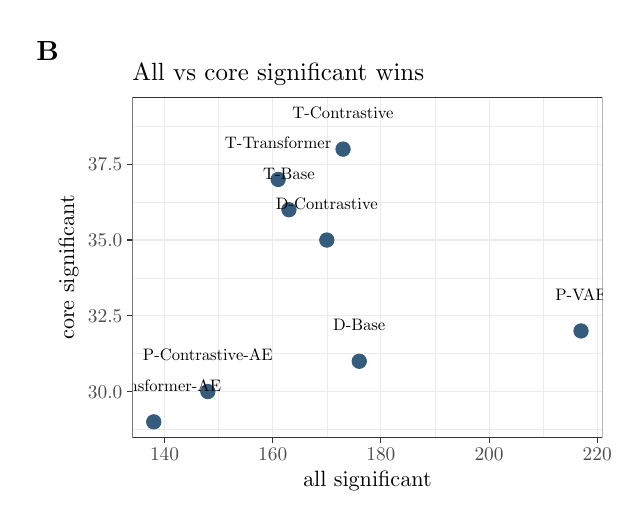
\begin{tikzpicture}[x=1pt,y=1pt]
\definecolor{fillColor}{RGB}{255,255,255}
\path[use as bounding box,fill=fillColor,fill opacity=0.00] (0,0) rectangle (210.78,171.36);
\begin{scope}
\path[clip] (  1.11,  1.87) rectangle (209.67,169.49);
\definecolor{drawColor}{RGB}{255,255,255}
\definecolor{fillColor}{RGB}{255,255,255}

\path[draw=drawColor,line width= 0.4pt,line join=round,line cap=round,fill=fillColor] (  1.11,  1.87) rectangle (209.67,169.49);
\end{scope}
\begin{scope}
\path[clip] ( 37.84, 23.34) rectangle (207.67,146.20);
\definecolor{fillColor}{RGB}{255,255,255}

\path[fill=fillColor] ( 37.84, 23.34) rectangle (207.67,146.20);
\definecolor{drawColor}{gray}{0.92}

\path[draw=drawColor,line width= 0.2pt,line join=round] ( 37.84, 26.18) --
	(207.67, 26.18);

\path[draw=drawColor,line width= 0.2pt,line join=round] ( 37.84, 53.56) --
	(207.67, 53.56);

\path[draw=drawColor,line width= 0.2pt,line join=round] ( 37.84, 80.93) --
	(207.67, 80.93);

\path[draw=drawColor,line width= 0.2pt,line join=round] ( 37.84,108.31) --
	(207.67,108.31);

\path[draw=drawColor,line width= 0.2pt,line join=round] ( 37.84,135.68) --
	(207.67,135.68);

\path[draw=drawColor,line width= 0.2pt,line join=round] ( 69.01, 23.34) --
	( 69.01,146.20);

\path[draw=drawColor,line width= 0.2pt,line join=round] (108.10, 23.34) --
	(108.10,146.20);

\path[draw=drawColor,line width= 0.2pt,line join=round] (147.18, 23.34) --
	(147.18,146.20);

\path[draw=drawColor,line width= 0.2pt,line join=round] (186.27, 23.34) --
	(186.27,146.20);

\path[draw=drawColor,line width= 0.4pt,line join=round] ( 37.84, 39.87) --
	(207.67, 39.87);

\path[draw=drawColor,line width= 0.4pt,line join=round] ( 37.84, 67.25) --
	(207.67, 67.25);

\path[draw=drawColor,line width= 0.4pt,line join=round] ( 37.84, 94.62) --
	(207.67, 94.62);

\path[draw=drawColor,line width= 0.4pt,line join=round] ( 37.84,122.00) --
	(207.67,122.00);

\path[draw=drawColor,line width= 0.4pt,line join=round] ( 49.46, 23.34) --
	( 49.46,146.20);

\path[draw=drawColor,line width= 0.4pt,line join=round] ( 88.55, 23.34) --
	( 88.55,146.20);

\path[draw=drawColor,line width= 0.4pt,line join=round] (127.64, 23.34) --
	(127.64,146.20);

\path[draw=drawColor,line width= 0.4pt,line join=round] (166.73, 23.34) --
	(166.73,146.20);

\path[draw=drawColor,line width= 0.4pt,line join=round] (205.81, 23.34) --
	(205.81,146.20);
\definecolor{drawColor}{RGB}{53,92,125}
\definecolor{fillColor}{RGB}{53,92,125}

\path[draw=drawColor,line width= 0.3pt,line join=round,line cap=round,fill=fillColor] (113.96,127.47) circle (  2.61);

\path[draw=drawColor,line width= 0.3pt,line join=round,line cap=round,fill=fillColor] ( 90.51,116.52) circle (  2.61);

\path[draw=drawColor,line width= 0.3pt,line join=round,line cap=round,fill=fillColor] ( 94.41,105.57) circle (  2.61);

\path[draw=drawColor,line width= 0.3pt,line join=round,line cap=round,fill=fillColor] (108.10, 94.62) circle (  2.61);

\path[draw=drawColor,line width= 0.3pt,line join=round,line cap=round,fill=fillColor] (199.95, 61.77) circle (  2.61);

\path[draw=drawColor,line width= 0.3pt,line join=round,line cap=round,fill=fillColor] (119.82, 50.82) circle (  2.61);

\path[draw=drawColor,line width= 0.3pt,line join=round,line cap=round,fill=fillColor] ( 65.10, 39.87) circle (  2.61);

\path[draw=drawColor,line width= 0.3pt,line join=round,line cap=round,fill=fillColor] ( 45.56, 28.92) circle (  2.61);
\definecolor{drawColor}{RGB}{0,0,0}

\node[text=drawColor,anchor=base,inner sep=0pt, outer sep=0pt, scale=  0.60] at (113.96,138.55) {T-Contrastive};

\node[text=drawColor,anchor=base,inner sep=0pt, outer sep=0pt, scale=  0.60] at ( 90.51,127.60) {T-Transformer};

\node[text=drawColor,anchor=base,inner sep=0pt, outer sep=0pt, scale=  0.60] at ( 94.41,116.65) {T-Base};

\node[text=drawColor,anchor=base,inner sep=0pt, outer sep=0pt, scale=  0.60] at (108.10,105.70) {D-Contrastive};

\node[text=drawColor,anchor=base,inner sep=0pt, outer sep=0pt, scale=  0.60] at (199.95, 72.85) {P-VAE};

\node[text=drawColor,anchor=base,inner sep=0pt, outer sep=0pt, scale=  0.60] at (119.82, 61.90) {D-Base};

\node[text=drawColor,anchor=base,inner sep=0pt, outer sep=0pt, scale=  0.60] at ( 65.10, 50.95) {P-Contrastive-AE};

\node[text=drawColor,anchor=base,inner sep=0pt, outer sep=0pt, scale=  0.60] at ( 45.56, 40.00) {P-Transformer-AE};
\definecolor{drawColor}{gray}{0.20}

\path[draw=drawColor,line width= 0.4pt,line join=round,line cap=round] ( 37.84, 23.34) rectangle (207.67,146.20);
\end{scope}
\begin{scope}
\path[clip] (  0.00,  0.00) rectangle (210.78,171.36);
\definecolor{drawColor}{gray}{0.30}

\node[text=drawColor,anchor=base east,inner sep=0pt, outer sep=0pt, scale=  0.70] at ( 34.24, 37.46) {30.0};

\node[text=drawColor,anchor=base east,inner sep=0pt, outer sep=0pt, scale=  0.70] at ( 34.24, 64.84) {32.5};

\node[text=drawColor,anchor=base east,inner sep=0pt, outer sep=0pt, scale=  0.70] at ( 34.24, 92.21) {35.0};

\node[text=drawColor,anchor=base east,inner sep=0pt, outer sep=0pt, scale=  0.70] at ( 34.24,119.59) {37.5};
\end{scope}
\begin{scope}
\path[clip] (  0.00,  0.00) rectangle (210.78,171.36);
\definecolor{drawColor}{gray}{0.20}

\path[draw=drawColor,line width= 0.4pt,line join=round] ( 35.84, 39.87) --
	( 37.84, 39.87);

\path[draw=drawColor,line width= 0.4pt,line join=round] ( 35.84, 67.25) --
	( 37.84, 67.25);

\path[draw=drawColor,line width= 0.4pt,line join=round] ( 35.84, 94.62) --
	( 37.84, 94.62);

\path[draw=drawColor,line width= 0.4pt,line join=round] ( 35.84,122.00) --
	( 37.84,122.00);
\end{scope}
\begin{scope}
\path[clip] (  0.00,  0.00) rectangle (210.78,171.36);
\definecolor{drawColor}{gray}{0.20}

\path[draw=drawColor,line width= 0.4pt,line join=round] ( 49.46, 21.34) --
	( 49.46, 23.34);

\path[draw=drawColor,line width= 0.4pt,line join=round] ( 88.55, 21.34) --
	( 88.55, 23.34);

\path[draw=drawColor,line width= 0.4pt,line join=round] (127.64, 21.34) --
	(127.64, 23.34);

\path[draw=drawColor,line width= 0.4pt,line join=round] (166.73, 21.34) --
	(166.73, 23.34);

\path[draw=drawColor,line width= 0.4pt,line join=round] (205.81, 21.34) --
	(205.81, 23.34);
\end{scope}
\begin{scope}
\path[clip] (  0.00,  0.00) rectangle (210.78,171.36);
\definecolor{drawColor}{gray}{0.30}

\node[text=drawColor,anchor=base,inner sep=0pt, outer sep=0pt, scale=  0.70] at ( 49.46, 14.92) {140};

\node[text=drawColor,anchor=base,inner sep=0pt, outer sep=0pt, scale=  0.70] at ( 88.55, 14.92) {160};

\node[text=drawColor,anchor=base,inner sep=0pt, outer sep=0pt, scale=  0.70] at (127.64, 14.92) {180};

\node[text=drawColor,anchor=base,inner sep=0pt, outer sep=0pt, scale=  0.70] at (166.73, 14.92) {200};

\node[text=drawColor,anchor=base,inner sep=0pt, outer sep=0pt, scale=  0.70] at (205.81, 14.92) {220};
\end{scope}
\begin{scope}
\path[clip] (  0.00,  0.00) rectangle (210.78,171.36);
\definecolor{drawColor}{RGB}{0,0,0}

\node[text=drawColor,anchor=base,inner sep=0pt, outer sep=0pt, scale=  0.80] at (122.75,  5.64) {all significant};
\end{scope}
\begin{scope}
\path[clip] (  0.00,  0.00) rectangle (210.78,171.36);
\definecolor{drawColor}{RGB}{0,0,0}

\node[text=drawColor,rotate= 90.00,anchor=base,inner sep=0pt, outer sep=0pt, scale=  0.80] at ( 16.80, 84.77) {core significant};
\end{scope}
\begin{scope}
\path[clip] (  0.00,  0.00) rectangle (210.78,171.36);
\definecolor{drawColor}{RGB}{0,0,0}

\node[text=drawColor,anchor=base west,inner sep=0pt, outer sep=0pt, scale=  0.90] at ( 37.84,152.18) {All vs core significant wins};
\end{scope}
\begin{scope}
\path[clip] (  0.00,  0.00) rectangle (210.78,171.36);
\definecolor{drawColor}{RGB}{0,0,0}

\node[text=drawColor,anchor=base,inner sep=0pt, outer sep=0pt, scale=  1.00] at (  7.20,159.49) {\bfseries B};
\end{scope}
\end{tikzpicture}
